\chapter{Deep Neural Networks}

The history of artificial neural networks (ANN) dates back to 1943. In \cite{McCulloch1943} authors tried to mathematically describe the activity of biological neurons in the human brain. Using these principles they built a first artificial neuron and artificial neural network. In 1974 a PhD student, Paul Werbos, introduced in \cite{Werbos1974} the idea of backpropagation of errors by which ANN are able to learn other than linearly separable problems, and this idea was further expanded in \cite{Rumelhart1986}. Artificial neural networks that contain many hidden layers are also called deep neural networks (DNN) and the process of training this network is called deep learning \cite{LeCun2015}. Over the years deep learning and one of its variants - convolutional neural network that was proposed in \cite{LeCun2015-2} - were found to be very effective and precise in domains that were found unreachable by the classical AI and ML algorithms \cite{LeCun2015}. This was caused by their ability to capture abstract and complex patterns that simpler models found impossible to catch. Such examples include analysis of image data \cite{Farabet2013, Alzubaidi2021} and recent advancements in natural language processing (NLP) \cite{Deng2018}.

\section{Structure}
The fundamental part of every artificial neural network is the neuron. Neuron is basically a function which has one or more inputs and one output. Inside of this neuron, a mathematical computation is being done in order to transform input into output. Input can also be referred to as input vector or vector of input features. Each input feature has its weight by which it is multiplied. Next a bias is added to the multiplied and summed features and weights. This calculation is still linear so in order for it to be able to capture more complex patterns, we need to apply non-linear activation function to its output. The mathematical representation of artificial neuron can be seen in the equation bellow:

\begin{align}
    z &= b + \sum_{i=1}^n (w_i x_i) \\
    a &= f(z)
\end{align}

Where $z$ is the output produced by the linear unit, $b$ is the bias, $n$ is the number of input features, $x_i$ is the \textit{i}-th input feature, $w_i$ is the weight associated with the \textit{i}-th input feature, $a$ is the actual output, and $f$ is the activation function.

Visual example of artificial neuron can be seen in figure \ref{fig:artificial-neuron}.

\begin{figure}[H]
\begin{centering}
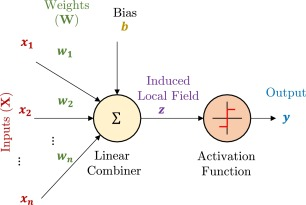
\includegraphics[width=8cm]{assets/images/neuron.jpg}
\par\end{centering}
\caption{Artificial neuron \cite{Santosh2022-1}}
\label{fig:artificial-neuron}
\end{figure}

\subsection{Activation Functions}
Activation functions are used to break linearity in neural networks - this enables them to capture more complex patterns, which are not linearly separable. Activation functions are used in combination with linear functions inside neurons. Different activation functions can be used, such as Sigmoid, Tanh, ReLU, ELU, GELU, and many more \cite{Dubey2022, Aby2025}.  The important part of an activation function is also its gradient, which is computed during backpropagation. 

\paragraph{Sigmoid}
Sigmoid is computed by the equation \ref{eq:sigmoid} and its derivative by the equation \ref{eq:sigmoid-derivative}. As we can see in figure \ref{fig:sigmoid} has a steep gradient around zero and it gradually flattens on both sides.

\begin{align}
\label{eq:sigmoid}
    \sigma(z) &= \frac{1}{1+e^{-z}} \\
\label{eq:sigmoid-derivative}
    \sigma^{'}(z) &= \sigma(z)(1-\sigma(z))
\end{align}

\begin{figure}[H]
\begin{centering}
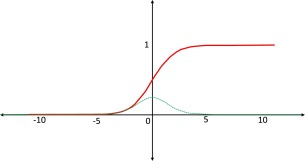
\includegraphics[width=8cm]{assets/images/sigmoid.jpg}
\par\end{centering}
\caption{Sigmoid activation function (red) and its derivative (green) \cite{Santosh2022-2}}
\label{fig:sigmoid}
\end{figure}

The output of the sigmoid is bound between zero and one, and its gradient can be used to push the output either closer to one or closer to zero \cite{Santosh2022-2}. It is often used for the output unit for the binary classification task, where the output is desired to be between zero and one \cite{Santosh2022-2, Goodfellow2016}.

\paragraph{Tanh} Next function is the \textit{tanh} activation function, given by the equation \ref{eq:tanh} and its respective derivative displayed on the equation \ref{eq:tanh-derivative}.

\begin{align}
\label{eq:tanh}
    \text{tanh}(z) &= \frac{e^z-e^{-z}}{e^z+e^{-z}} \\
\label{eq:tanh-derivative}
    \text{tanh}^{'}(z) &= 1-tanh^2(z)
\end{align}

Like the \textit{sigmoid} function, it compresses the input; however, unlike the \textit{sigmoid}, its output is constrained to the range of -1 to 1, as shown in figure \ref{fig:tanh}.

\begin{figure}[H]
\begin{centering}
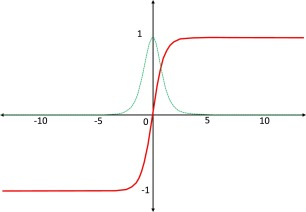
\includegraphics[width=8cm]{assets/images/tanh.jpg}
\par\end{centering}
\caption{Tanh activation function (red) and its derivative (green) \cite{Santosh2022-2}}
\label{fig:tanh}
\end{figure}

\paragraph{ReLU}
The problem with \textit{sigmmoid} and \textit{tanh} functions is the vanishing gradient and computational complexity. Vanishing gradient means that the gradient of a function is almost flat, hence close to zero, which leads to no or very little update in the network's learnable parameters (weights and biases) during the training \cite{Dubey2022, Aby2025}.

As a possible solution to these problems, a rectified linear unit, also known as ReLU, was introduced \cite{Nair2010}. ReLU is a simple function; its equation \ref{eq:relu} and derivative equation \ref{eq:relu-derivative} are straightforward.

\noindent
\begin{multicols}{2} % Two-column layout
    \begin{equation}
    \text{ReLU}(z) =
    \begin{cases} 
        z, & \text{if } z > 0, \\
        0, & \text{if } z \leq 0.
    \end{cases}
    \label{eq:relu}
    \end{equation}

    \begin{equation}
    \text{ReLU}'(z) =
    \begin{cases} 
        1, & \text{if } z > 0, \\
        0, & \text{if } z \leq 0.
    \end{cases}
    \label{eq:relu-derivative}
    \end{equation}
\end{multicols}

The ReLU function can be seen in figure \ref{fig:relu}. It basically returns its input if the input is positive otherwise, it returns zero. Since the derivative of \textit{x} is always one, the problem with vanishing gradient is solved. 

\begin{figure}[H]
\begin{centering}
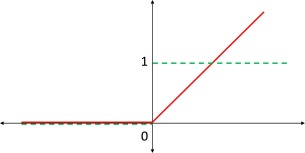
\includegraphics[width=8cm]{assets/images/relu.jpg}
\par\end{centering}
\caption{ReLU activation function (red) and its derivative (green) \cite{Santosh2022-2}}
\label{fig:relu}
\end{figure}

ReLU also introduces some potential drawbacks, i.e. the output for negative input is always zero. The problem called dying ReLU \cite{Dubey2022, Santosh2022-2, Aby2025} is when a negative input causes no updates in weights during training  and neurons in this state do not respond to error variations \cite{Santosh2022-2}. To fix this problem we can multiply the negative input value by a very small constant, which will allow the weights to be updated if it is needed. This modified ReLU is called Leaky ReLU \cite{Maas2013} and its formula and formula of its gradient are displayed on equations \ref{eq:leaky-relu} and \ref{eq:leaky-relu-derivative} respectively.

\noindent
\begin{multicols}{2} % Two-column layout
    \begin{equation}
    \text{LeakyReLU}(z) =
    \begin{cases} 
        z, & \text{if } z > 0, \\
        \alpha z, & \text{if } z \leq 0.
    \end{cases}
    \label{eq:leaky-relu}
    \end{equation}

    \begin{equation}
    \text{LeakyReLU}'(z) =
    \begin{cases} 
        1, & \text{if } z > 0, \\
        \alpha, & \text{if } z \leq 0.
    \end{cases}
    \label{eq:leaky-relu-derivative}
    \end{equation}
\end{multicols}

In addition to the Leaky ReLU, many other ReLU variants were introduced over the years, each bringing its own advantages, disadvantages, and challenges \cite{Dubey2022, Aby2025}.

Nowadays, the most commonly used activation function for hidden units is the ReLU activation function \cite{Dubey2022, Goodfellow2016}.
% overview, traditional, new 

\subsection{Layers}

Similarly to biological neural networks, when artificial neurons are chained together, meaning the output from one neuron is passed to another neuron, they create an artificial neural network.

This network is organized in layers. Neurons in each layer are not connected together, but rather every neuron from layer \textit{L} is connected with every neuron from layer \textit{L+1}, except neurons in the first (input) layer. For better understanding, we will refer to the figure \ref{tab:artificial-nn} where we can see an example of a neural network.

\begin{figure}[H]
\begin{centering}
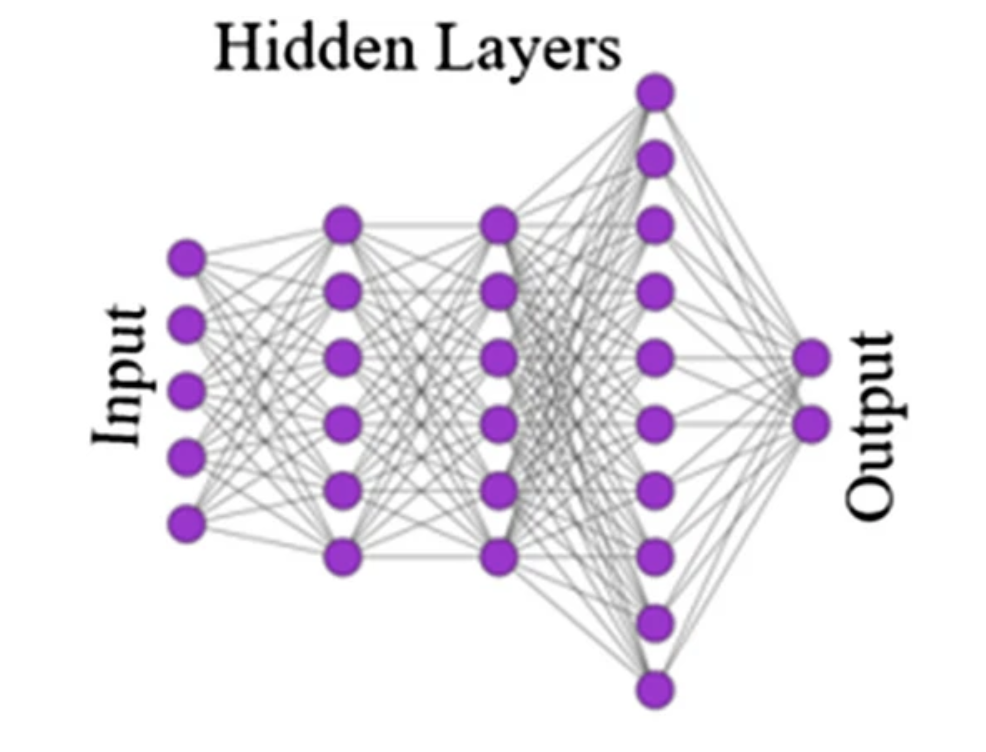
\includegraphics[width=8cm]{assets/images/neural_net.png}
\par\end{centering}
\caption{Example of deep artificial neural network \cite{TalaeiKhoei2023}}
\label{tab:artificial-nn}
\end{figure}

Neural network can be split into three main parts:

\begin{itemize}
    \item Input layer
    \item Hidden layers
    \item Output layer
\end{itemize}

Input layer is the initial layer and the only layer that does not contain neurons which perform calculations but rather consists of \textit{N} input features $x_1, x_2, \dots, x_N$ also referred to as a vector $\vec{x}$ of input features:

\[
\vec{x} = \begin{bmatrix}
x_1 \\
x_2 \\
\vdots \\
x_N
\end{bmatrix}
\]

The subsequent layers between the input layer and output layer are called hidden layers. The name comes from the fact that their outputs are not directly observable, nor are they provided by the external environment - they are internal to the network's architecture. Neurons inside these layers perform calculations on the input and produce output, which is then fed forward to the next layer.

The final output layer produces an output of the network. Output and number of neurons depend on the task the network is being trained for. For regression task one neuron is often suitable - it predicts a continuous variable \cite{Goodfellow2016}. During classification task it can further depend on the nature of the classification. In binary classification, again a single neuron can suffice. It will display a probability of the input belonging to one of the classes - if the probability is high, it will assign that class to it, and if the probability is low, it will assign the other class to it \cite{Goodfellow2016}. In multi-class classification, the number of neurons is the same as the number of classes and each neuron predicts a probability of the input belonging to one specific class \cite{Goodfellow2016}.

%TODO: input, hidden, output layer, deep nn, image

\section{Loss Functions}

\section{Training}

\subsection{Forward Propagation}

\subsection{Backpropagation}

\subsection{Hyperparameters}

\section{Evaluation Metrics}

\section{Architectures}